\documentclass{patmorin}
\usepackage{amsthm,graphicx}
\usepackage{pat}

\newcommand{\HH}{\mathcal{H}}
\renewcommand{\div}{\mathop{\mathrm{div}}}

\title{Notes on Multiplicative Hashing}
\author{Pat Morin}

\begin{document}
\maketitle
This document contains some notes on work done with Dana, Sander, and
Nima on the subject of multiplicative hashing.

We consider the hash function family
\[
   \HH = \{ h_z(x) = (zx\bmod 2^w) \div 2^{w-d} : z \in\{1,3,\ldots,2^w-1 \} \}
\]
which maps $w$-bit integers onto $d$-bit integers. 
We can think of $z$ as a sequence of $w-1$ random bits followed by a 1.
This function is 2-universal in the sense that, for any distinct $x,y\in
\{0,\ldots,2^w\}$ and a random $h\in\HH$, $\Pr\{h(x)=h(y)\} \le 2/2^d$
(Dietzfelbinger \etal\ 1997).


For an integer $x$, we denote the $i$th bit in the binary representation of $x$ by $x_i$, so that $x=\sum_{i=0}^\infty 2^ix_i$.   We also $\langle x_k,\ldots,x_0\rangle=\sum_{i=0}^k 2^ix_i$.
With these notations, $h_z(x) = \langle (zx)_{w-1},\ldots,(zx)_{w-d}\rangle$.


\section{The Lower Bound}
My first question was about whether the upper bound on the collision
probability was tight.  The answer is yes:
\begin{clm}
  For a random $h\in\HH$, $\Pr\{h(2^{w-d-2}) = h(3\cdot2^{w-d-2})\}
   = 2/2^d$.
\end{clm}

\begin{proof}
\[ h(2^{w-d-2}) = (z_{d+1},\ldots,z_{2})_2 \]
\begin{eqnarray*} h(3\cdot 2^{w-d-2}) 
  &=& ((z_{d+1},\ldots,z_{0})_2  +  (z_{d},\ldots,z_{0},0)_2) \div 4 \\
  &=& ((z_{d+1},\ldots,z_1,1)_2  +  (z_{d},\ldots,z_1,1,0)_2) \div 4 \\
  &=& ((z_{d+1},\ldots,z_1)_2  +  (z_{d},\ldots,z_1,1)_2) \div 2 \\
  &=& (t_d,\ldots,t_0)_2
\end{eqnarray*}
Suppose that the first equation equals the second equation.
If $z_1=1$, then $t_0 = (1+z_1+z_2)\bmod 2 = z_2$ and the overflow carries into $t_1$, giving $t_1 = (1+z_2+z_3)\bmod 2 = z_3$, so that $z_2=1$.  This in turn carries into $t_2$, yielding the equations
\[
   1=z_2=z_3=\cdots=z_d
\]
which are only satisfied with probability $1/2^{d-1}$.

If $z_1=0$, then $t_0=(z_1+z_2)\bmod 2 = z_3$, so that $z_2=0$.  The same
reasoning as above leads to the equations
\[
   0=z_2=z_3=\cdots=z_d
\]
which are only satisfied with probability $1/2^{d-1}$.
\end{proof}

\section{Other Bounds}

This picture shows the collisions probabilities of $x$ and $y$ when $w=9$
and $d=1$.

\noindent 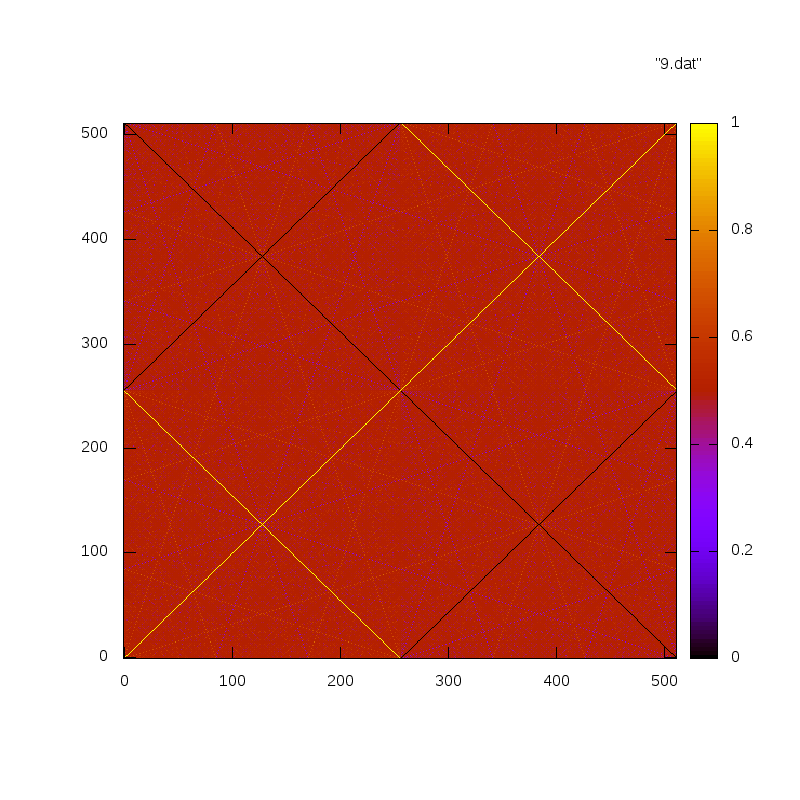
\includegraphics[width=\textwidth]{9}

Here are some observations:

\begin{clm}\clmlabel{negater}
For $d=1$, $\Pr\{h(x)=1\} = \Pr\{h(x+2^{w-1})=0\}$
\end{clm}

\begin{proof}
$h(x)$ and $h(x+2^{w-1})$ are the complement of each other because
\[ h(x+2^{w-1}) = (z(x+2^{w-1}))_{w-1} = (zx + z2^{w-1})_{w-1} = \neg(zx)_{w-1} = \neg h(x)
\]
where the last equality follows because $z$ is odd.
\end{proof}

\begin{clm}
For $d=1$, $\Pr\{h(x) = h(-x + 2^{w-1})\} = 1$, except for $x=0$
or $x=2^{w-1}$.
\end{clm}

\begin{proof}
Negating $x$ is equivalent to negatings its bits and adding 1, so
\[
   -zx = \langle\neg{(zx)_{w-1}},\ldots,\neg{(zx)_{0}}\rangle + 1 
        \stackrel{\mathrm{def}}{=} \langle t_{w-1},\ldots,t_0\rangle
\]
Observe that the conditions imposed on $x$ imply that $t_{w-1}=\neg{(zx)_{w-1}}$.  Finally, observe that, by \clmref{negater}, $h(-x+2^{w-1})=\neg{t_{w-1}}=(zx)_{w-1}= h(x)$.
\end{proof}

\begin{clm}\clmlabel{3x}
For $d=1$, $\Pr\{h(x) = h(3x)\} > 1/2$.\footnote{Experiments show that this probability is actually $2/3$.}
\end{clm}

\begin{proof}
Since $z3x=2zx + zx$, we have
\[
z3x\bmod 2^w =
\begin{array}{rrrrrrrrrr}
& \langle & (zx)_{w-1}& (zx)_{w-2}& \ldots&(zx)_1&(zx)_0 & \rangle \\ 
+& \langle & (zx)_{w-2}& (zx)_{w-3}&\ldots&(zx)_0& 0 & \rangle  
\end{array}
\]
If $(zx)_{w-2} = 1$, then $\Pr\{h(x)=h(3x)\}$ is equal to the probability
that an overflow bit is carried from position $w-2$ into position $w-1$,
conditional on $(zx)_{w-2} = 1$.  This event occurs if $z_{w-3}=1$
or an overflow bit is carried from position $w-3$ into position $w-2$.
Clearly this probability is greater than $1/2$.

On the other hand, if $(zx)_{w-2} = 0$ then $\Pr\{h(x)=h(3x)\}$ is equal
to the probability that no overflow bit is carried from position $w-2$
into position $w-1$, conditional on $(zx)_{w-2} = 0$.  This event occurs
if $z_{w-3}=0$ or no overflow bit is carried from position $w-3$ into
position $w-2$.  Clearly this probability is greater than $1/2$.
\end{proof}

\begin{clm}
For $d=1$, $\Pr\{h(x)=h(-3x)+2^{w-1}\} > 1/2$.
\end{clm}

\begin{proof}
This is an easy combination of the arguments used in the proofs of \clmref{3x} and \clmref{negater}.
\end{proof}

These picture shows the collisions probabilities of $x$ and $y$ when $w=9$
and $d=2,3,4$.

\noindent 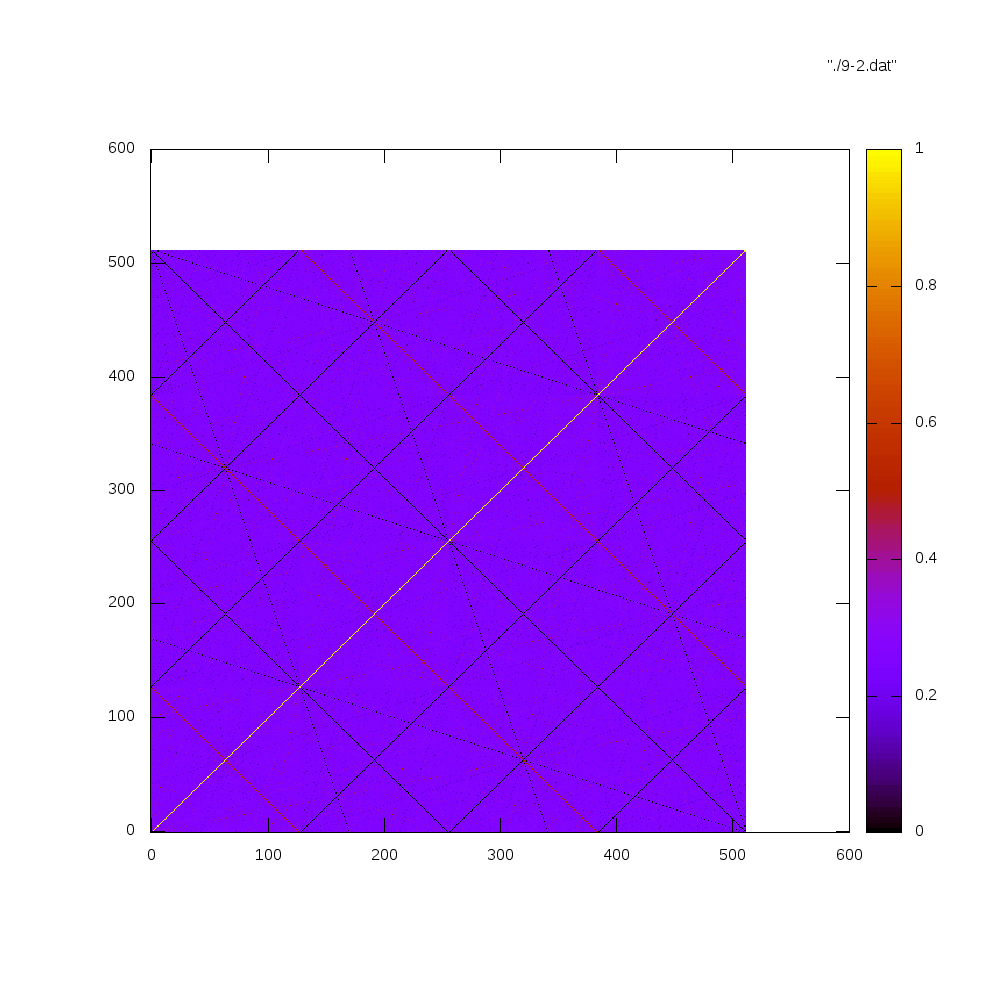
\includegraphics[width=\textwidth]{9-2}

\noindent 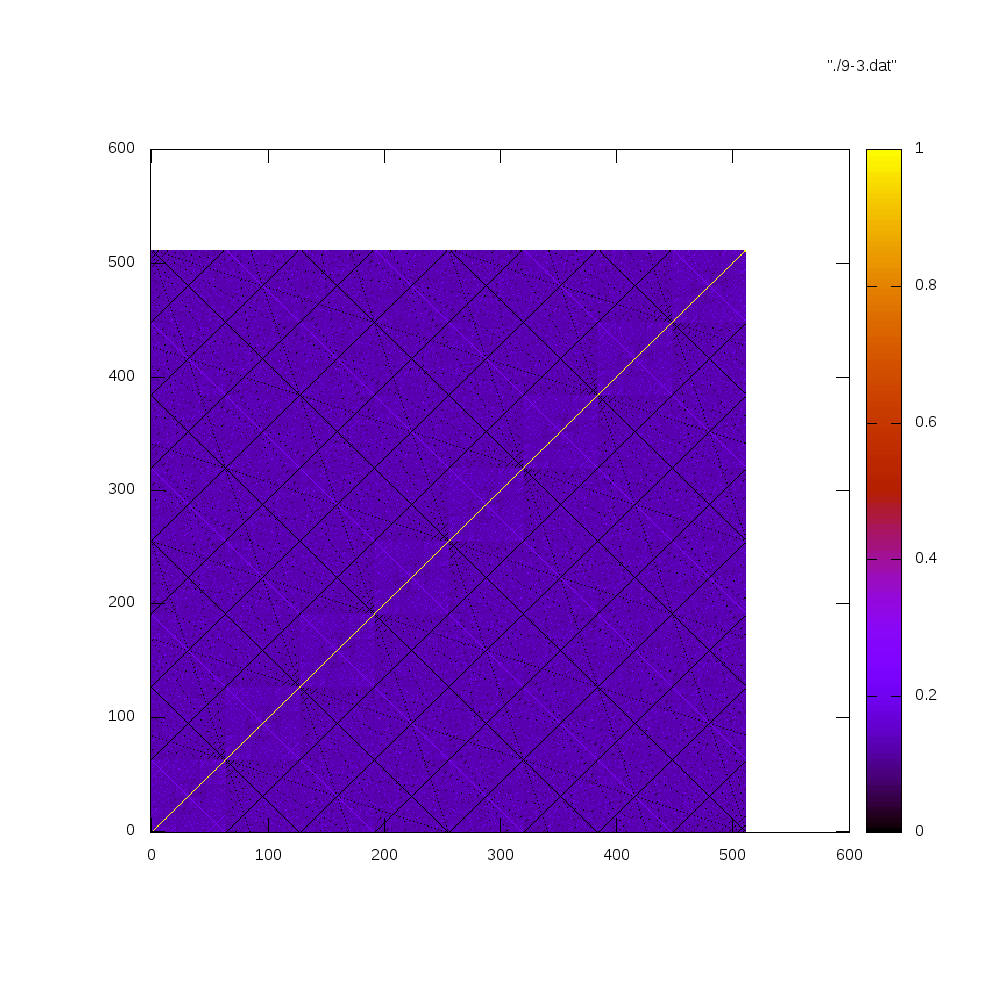
\includegraphics[width=\textwidth]{9-3}

\noindent 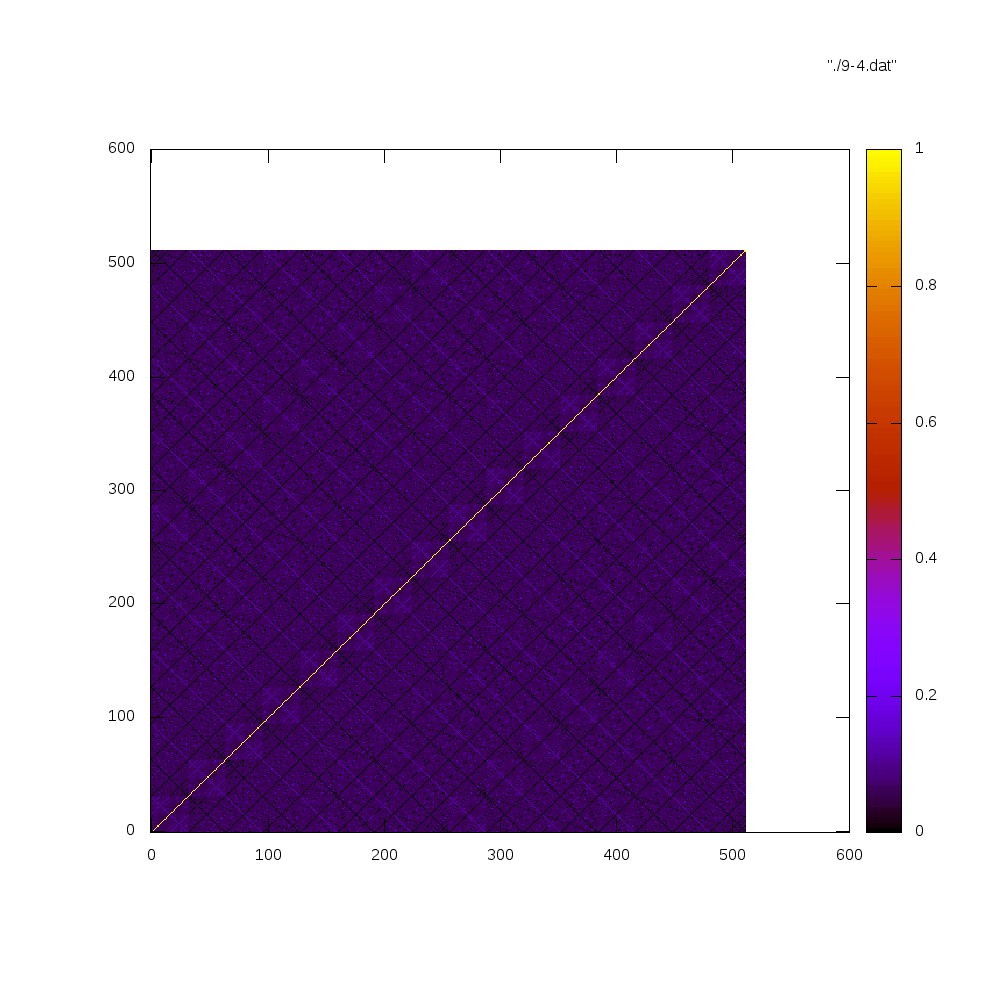
\includegraphics[width=\textwidth]{9-4}



\end{document}
